\documentclass[a4paper,11pt]{article}
\usepackage[american]{babel}
\usepackage[utf8]{inputenc}
\usepackage{geometry}
\usepackage{booktabs}  
\usepackage{graphicx} 
\usepackage{listings}
\usepackage{amsmath,amsthm,amssymb}
\lstset{%
backgroundcolor=\color{cyan!10},
basicstyle=\ttfamily,
numbers=left,numberstyle=\scriptsize
}
\setlength{\parindent}{0cm}
\usepackage[wby]{callouts}

\title{Memoria Práctica 3}
\author{Álvaro Beltrán}
\begin{document}

\maketitle
\begin{center}
Grupo 3, Ofelia Retamero Pascual
\end{center}

\begin{figure}[h]

\includegraphics[scale=0.3]{UGR}
\centering
\end{figure}

\newpage

\renewcommand*\contentsname{Índice}
\tableofcontents

\newpage

\section{Introducción}
Este ejercicio se centra en el ajuste de un modelo lineal a dos conjuntos de datos dados con el
objetivo de obtener el mejor predictor posible. En todos los casos los pasos a desarrollar serán
aquellos que nos conduzcan al ajuste y selección del mejor modelo y a la estimación del error
Eout del modelo final.

\section{Base de datos OptDigits}

\subsection{Comprensión del problema}

Nos encontramos ante una base de datos sobre manuscritos de dígitos (0..9), en la cual contamos con 5620 instancias etiquetadas. Las instancias cuentan con 64 atributos más la etiqueta, cada atributo es un entero del 0 al 16 y cada etiqueta representa el dígito que es (del 0 al 9). Para generar los atributos se cogieron bitmaps de manuscritos de los dígitos de 32x32 pixeles, estos se dividieron en celdas de 4x4 para conseguir disminuir la dimensionalidad a 8x8 (64 atributos) cada celda de la matrix 8x8 se representa con un entero del 0 al 16 por que así conseguimos barrer todas las posibles celdas.\\

Por lo que tenemos que X son los 64 atributos de las instancias e Y son las etiquetas de las instancias. La función f que buscamos es la función que ante un bitmap de un manuscrito nos asigne un dígito.\\

Nos encontramos ante un problema de aprendizaje supervisado ya que tenemos todas las instancias etiquetadas. Como el objetivo del problema es decir a que clase (dígito del 0 al 9) pertenece un bitmap dado nos encontramos ante un problema de clasificación. \\

Para intentar entender la distribución de los datos he realizado una proyección al plano 2D con el algoritmo PCA para hacer un mapa de calor del conjunto:\\

\begin{figure}[h]
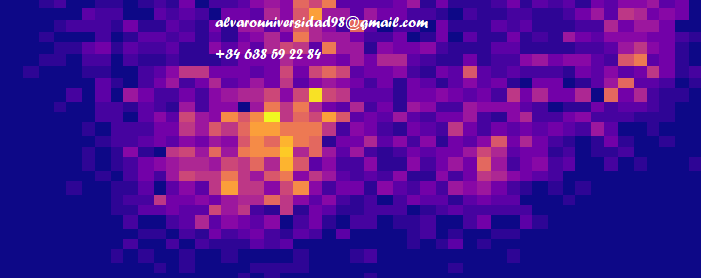
\includegraphics[scale=0.63]{heatmap}
\centering
\end{figure}

Al analizar esta representación no obtenemos gran información lo único que con esta reducción de dimensionalidad tenemos gran número de instancias en la parte inferior izquierda. 

\subsection{Selección clase de funciones}

Una de las clases de funciones que vamos a escoger es el hiperplano porque es la clase de funciones más simple posible que tiene en cuenta todos los atributos, para ello usamos el siguiente vector de características: $\Phi_1=(1,x_1,x_2,...,x_{63},x_{64})$.\\

También vamos a estudiar los resultados con las clases polinómicas de orden dos cuyo vector de características se construye de la siguiente forma: $(1+a+b)^2=1+a+b+a^2+b^2+ab$ (para dos atributos), en nuestro caso tenemos 64 y lo haremos con una función de sklearn (polynomial features). Elijo esta función para probar algo diferente a las lineales pero lo suficientemente simple para no crear overffiting, también hay que tener en cuenta la computabilidad de subir el grado. De hecho tras algunas pruebas si no reduzco las características al intentar ajustar una función de grado 3 mi ordenador no es capaz de computar cual quier algoritmo debido al número de atributos generados.

\subsection{Fijar los conjuntos de training y test}

En cuanto a los conjuntos he fijado uno de training y otro de test con el 80 y 20 porciento de los datos respectivamente, la base de datos viene con dos conjuntos predefinidos, para no dejarme guiar por su elección he unido ambos conjuntos, los he barajado y posteriormente he escogido los dos conjuntos ya nombrados.\\

El conjunto de training lo voy a usar para entrenar los modelos elegidos usando crossvalidation (CV) para elegir el mejor de todos ellos. Y con el conjunto de test veré un error aproximado de ese modelo.

\subsection{Preprocesamiento de los datos}

Primero cabe mencionar que la base de datos que hemos conseguido ya viene con un preprocesamiento hecho para reducir la dimensionalidad del bitmap de 32x32 a 8x8 (64 atributos), para ello hace lo que he explicado en la sección 2.1 .\\

Luego yo voy a aplicar una serie de técnicas de preprocesado de datos para mejorar los resultados al ajustar el modelo. Primero aplico \textbf{VarianceThreshold} que es una forma de eliminar caracacterísticas que aporten poca información estudiando la varianza, esto lo aplico por que supongo que algunas características como por ejemplo las asociadas a las esquinas serán mayoritariamente cero y no aportan información.Luego he aplicado \textbf{Polynomial Features} para trabajar con vectores de características de grados 1 y 2.\\ 

Por último he aplicado \textbf{StandardScaler} que es un estandarizado para que los valores se reescalen a $[0,1]$ por que regresión logística funciona mejor en este rango de valores al usar técnicas como el gradiente descendiente.

\subsection{Métrica}

Para este problema he elegido precisión (Accuracy) por que entiendo que cuando estamos clasificando un número lo que buscamos es no equivocarnos a la hora de hacer una predicción sobre a que clase pertenece.

\subsection{Técnica de ajuste elegida}

Para saber que técnica de ajuste debo elegir voy a probar con varias: perceptron, Newton y LBFGS.

\begin{itemize}
\item Perceptron por que es la técnica de ajuste típica en clasificación.
\item Newton por que calcula el learning rate que hay que in aplicando, siendo una mejora del SGD.
\item FBFGS por que es una mejora de Newton que aunque no la hayamos dado en clase viene implementada en scikit-learn e investigando un poco vemos que se usa para funciones complicadas y muchos atributos por su eficiencia en memoria cosa que nos interesa mucho en este problema.
\end{itemize}

\subsection{Regularización}

En cuanto a regularización he usado LASSO por que entiendo que hay características que no aportan información, como ya nombré antes las esquinas de la imagen por ejemplo.\\

En el script he realizado dos pruebas una con regularización y otra sin ella para ver la diferencia, vemos como el error dentro de la muestra sin aplicar LASSO es nulo por lo que es casi seguro que se haya producido overffiting, tras aplicar LASSO podemos comprobar que el error dentro de la muestra aumenta un poco, por lo que podemos afirmar que conseguimos reducir el overfitting.\\

No uso regularización de RIDGE por que no tengo suficiente información para afirmar que hay atributos correlados.

\subsection{Modelos}

Voy a usar dos modelos con distintos parámetros a estudiar cada uno:

\begin{itemize}
\item PLA-Pocket, voy ha escoger este modelo con perceptron y dos clases de funciones, de grado 1 y 2. Vamos a entrenar el modelo por defecto sin penalización l1 o l2.
\item Regresión logística, voy a ajustar con tres algoritmos: newton y FBFGS a la vez que hacemos inferencia sobre el grado 1 y 2, y sobre el parámetro C que es la potencia con la que aplicamos penalización l2.
\end{itemize}

En definitiva las posibles posibilidades que considero y el número que asigna GridSearchCV es:

\begin{table}[h]
\begin{tabular}{|l|c|c|c|c|}
\hline
Índice & \multicolumn{1}{l|}{Modelo}              & \multicolumn{1}{l|}{Técnica} & \multicolumn{2}{l|}{Hiperparámetros} \\ \hline
0      & \multicolumn{1}{l|}{Regresión Logística} & LBFGS                        & C=0.001          & Degree=1          \\ \hline
1      & Regresión Logística                      & LBFGS                        & C=0.001          & Degree=2          \\ \hline
2      & Regresión Logística                      & Newton                       & C=0.001          & Degree=1          \\ \hline
3      & Regresión Logística                      & Newton                       & C=0.001          & Degree=2          \\ \hline
4      & Regresión Logística                      & LBFGS                        & C=1.0            & Degree=1          \\ \hline
5      & Regresión Logística                      & LBFGS                        & C=1.0            & Degree=2          \\ \hline
6      & Regresión Logística                      & Newton                       & C=1.0            & Degree=1          \\ \hline
7      & Regresión Logística                      & Newton                       & C=1.0            & Degree=2          \\ \hline
8      & Regresión Logística                      & LBFGS                        & C=1000           & Degree=1          \\ \hline
9      & Regresión Logística                      & LBFGS                        & C=1000           & Degree=2          \\ \hline
10     & Regresión Logística                      & Newton                       & C=1000           & Degree=1          \\ \hline
11     & Regresión Logística                      & Newton                       & C=1000           & Degree=2          \\ \hline
12     & PLA-Pocket                               & Perceptron                   & \multicolumn{2}{c|}{Degree=1}        \\ \hline
13     & PLA-Pocket                               & Perceptron                   & \multicolumn{2}{c|}{Degree=2}        \\ \hline
\end{tabular}
\end{table}

\subsection{Estimación de hiperparámetros y selección del mejor modelo.}

Para seleccionar el mejor modelo y estimar los hiperparámetros anteriormente mencionados he usado una función de scikit-learn llamada GridSearchCV donde podemos definir los modelos que vamos a usar, la métrica para el error, el número de conjuntos para validación cruzada y los parámetros sobre los que vamos a hacer inferencia, para hacer todo ello también usamos un Pipeline.\\

He realizado dos entrenos uno con regularización y otro si regularización para poder ver si se producía overffiting.\\

Sin regularización obtenemos que el mejor modelo es regresión logística con LBFGS. Esta función lo que hace es elegir el mejor modelo usando validación cruzada, escogiendo el modelo que en media mejores resultados ha obtenido de las subdivisiones del conjunto de training estudiando el error asociado a la precisión (Accuracy). Los resultados del entreno son los siguientes:\\

\newpage

\begin{table}[h]
\begin{tabular}{|l|l|l|l|}
\hline
Índice     & rank\_test\_score & mean\_fit\_time    & mean\_test\_score \\ \hline
0          & 13                & 0.171139           & 0.877890          \\ \hline
1          & 10                & 6.073368           & 0.949956          \\ \hline
2          & 14                & 0.346274           & 0.877668          \\ \hline
3          & 10                & 17.973353          & 0.949956          \\ \hline
4          & 6                 & 1.309494           & 0.969753          \\ \hline
\textbf{5} & \textbf{1}        & \textbf{41.043083} & \textbf{0.987545} \\ \hline
6          & 6                 & 1.579378           & 0.969753          \\ \hline
\textbf{7} & \textbf{1}        & \textbf{50.502794} & \textbf{0.987545} \\ \hline
8          & 8                 & 4.036009           & 0.957074          \\ \hline
9          & 4                 & 6.450557           & 0.985544          \\ \hline
10         & 9                 & 3.681363           & 0.956852          \\ \hline
11         & 3                 & 15.986265          & 0.985989          \\ \hline
12         & 12                & 0.593810           & 0.946178          \\ \hline
13         & 5                 & 5.709131           & 0.978648          \\ \hline
\end{tabular}
\end{table}

Como podemos ver tenemos dos algoritmos que dan la misma precisión en media, pues Newton y LBFGS es lo mismo con la diferencia de que LBFGS tiene optimización de memoria, por eso este último consigue hacerlo en menos tiempo y es el modelo elegido con los siguientes parámetros:

\begin{table}[h]
\begin{tabular}{|c|c|c|c|}
\hline
\textit{\textbf{Modelo}} & \textit{\textbf{Solver}} & \textit{\textbf{C}} & \textit{\textbf{Polynomial Degree}} \\ \hline
Regtresión Logistica     & LBFGS                    & 1.0                 & 2                                   \\ \hline
\end{tabular}
\end{table}

Con estos parámetros obtenemos una precisión dentro de la muestra del 100$\%$ por lo que como no hemos realizado regularización podemos sospechar que se ha producido overffiting. Sin embargo, tenemos que la precisión en el conjunto de test que no hemos usado en el entreno es de 98.843$\%$.  \\

Cuando añadimos al preprocesamiento de los datos regularización LASSO conseguimos como resultado los mismos parámetros y la precisión disminuye. Una precisión dentro de la muestra del 99.866$\%$ y una precisión en el conjunto de test de 96.708$\%$.



\subsection{Error producido al estimar el Modelo}

En el siguiente gráfico muestro los errores obtenidos en cada una de las subdivisiones de train hechas sin regularización:
\newpage
\begin{figure}[h]
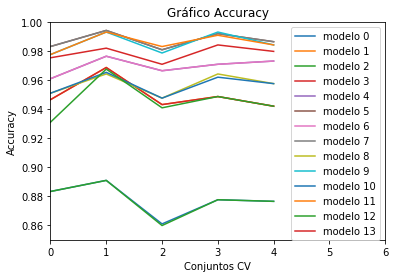
\includegraphics[scale=0.6]{errores}
\centering
\end{figure}

Podemos ver como excepto uno todos superan el 90$\%$ de precisión. Y los dos modelos nombrados anteriormente son los que obtienen los mejores resultados (los modelos 5 y 7).\\

Sin embargo, cuando hacemos regularización notamos un descenso de la Precisión generalizado aunque los dos modelos mejores sigan siendo los mismos:

\begin{figure}[h]
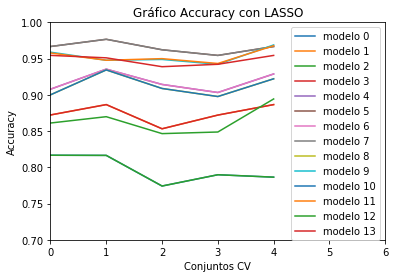
\includegraphics[scale=0.6]{erroresLasso}
\centering
\end{figure}

En cuanto a los errores en nuestro conjunto reservado para test vemos como en el primer caso tenemos un error del 98.843$\%$ y tras aplicar regularización tenemos un 96.708$\%$, por lo que podemos decir que la regularización no ha funcionado como debía.

\subsection{Justificación}

El modelo elegido representa de forma adecuada los datos tal y como se refleja en el error producido en los datos que no hemos usado. Aunque no puedo asegurar que mi modelo sea el mejor posible, ya que esta afirmación es imposible, si que es una cota muy buena, la cual parece muy difícil mejorar.\\

Aún así creo que he barrido una gran variedad de modelos de los cuales el que he seleccionado es el mejor de ellos. Aplicando validación cruzada que es una técnica muy interesante y muy eficaz en la elección del mejor modelo, debido a que entrenamos y obtenemos errores de diferentes conjuntos y luego estudiamos la media de error de cada modelo, consiguiendo así una mejor adaptación a otros conjuntos de la base de datos. Por lo que puedo decir que por todos los resultados obtenidos hemos conseguido un muy buen modelo que ajusta fielmente los datos.\\

A parte considero que el preprocesamiento elegido es crucial para que regresión logística funcione tan bien, es decir, eliminamos algunas características que no aportan información para que compute mejor los datos. Además de la estandarización que realizamos para escalar los datos entre [0,1] cosa que ayuda enormemente tanto al problema de clasificación como a la aplicación de la regresión logística.


\section{Communities and Crime Data Set}

\subsection{Comprensión del problema}

Nos encontramos ante un problema de regresión que estudia predecir el crimen en las comunidades estadounidenses. La base de datos aporta datos socio-económicos del censo de 1990, el cumplimiento de la ley en 1990 datos del crimen en 1995. La base de datos aporta 1994 instancias y estudia 127 atributos, añadiendo un último atributo al final con la etiqueta que determina el número de crímenes violentos por cada 10000 habitantes.\\

Todos los atributos son numéricos (números reales) excepto uno que aporta el nombre de las ciudades. La definición de lo que estudia cada uno de los atributos se encuentra en "communities.data".

\begin{figure}[h]
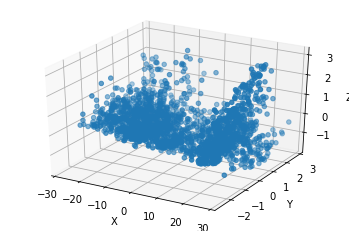
\includegraphics[scale=0.6]{datoscom}
\centering
\end{figure}

En el gráfico de arriba vemos una proyección al plano 3D realizada con PCA, pero como vemos no aporta mucha información.

\subsection{Selección clase de funciones}

Una de las clases de funciones que vamos a escoger es el hiperplano porque es la clase de funciones más simple posible que tiene en cuenta todos los atributos, para ello usamos el siguiente vector de características: $\Phi_1=(1,x_1,x_2,...,x_{126},x_{127})$.\\

También vamos a estudiar los resultados con las clases polinómicas de orden dos ya explicadas en la sección 2.2 .

\subsection{Fijar los conjuntos de training y test}

En cuanto a los conjuntos he fijado uno de training y otro de test con el 80 y 20 porciento de los datos respectivamente, los he barajado y posteriormente he escogido los dos conjuntos ya nombrados.\\

El conjunto de training lo voy a usar para entrenar los modelos elegidos usando crossvalidation (CV) para elegir el mejor de todos ellos. Y con el conjunto de test veré un error aproximado de ese modelo.

\subsection{Preprocesamiento de los datos}

Primero cabe mencionar que la base de datos nos dice que los cinco primeros atributos son non-predictive por los que los elimino.\\

También podemos ver como hay muchos datos perdidos en la base de datos, por lo que aplico una técnica para rellenar los valores perdidos con la media.\\

Luego yo voy a aplicar una serie de técnicas de preprocesado de datos para mejorar los resultados al ajustar el modelo. Primero aplico \textbf{VarianceThreshold} que es una forma de eliminar caracacterísticas que aporten poca información estudiando la varianza. He aplicado también \textbf{Polynomial Features} para trabajar con vectores de características de grados 1 y 2. Por último he aplicado \textbf{StandardScaler} que es un estandarizado para que los valores se reescalen a $[0,1]$.

\subsection{Métrica}

Para este problema he elegido el error cuadrático medio para estudiar el error en la predicción. Por que aparte de ser la función más simple y más usada como hemos rellenado los valores perdidos con la media, buscamos que estos valores no afecten mucho.

\subsection{Técnica de ajuste elegida}

En cuanto a las técnicas que uso son Gradiente Descendiente Estocástico (SGD) y pseudoinversa. Gradiente Descendiente Estocástico lo uso en un modelo de regresión lineal común de mínimos cuadráticos y pseudoinversa en otros 3 tipos de modelos. Cuando uso pseudoinversa dejo el modelo de resolución del sistema en default, por que así selecciona dependiendo del tipo de datos que tenemos el modelo de resolución óptimo. 

\subsection{Regularización}

Regularización es uno de los hiperparámetros sobre los que he hecho inferencia, uno de los modelos no hace regulariación, en los otros tres si hago. En uno de ellos comparo las regularizaciones l1 y l2 para elegir la que obtiene mejores resultados. En cuanto a los dos últimos modelos cada uno de ellos lleva por defecto l1 y l2 respectivamente, de forma que escojer un modelo de ellos significa escoger ese tipo de regularización.

\subsection{Modelos}

voy a usar cuatro modelos con diferentes parámetros sobre los que hacer inferencia en cada uno:

\begin{itemize}
\item SGDRegresor. Que es un algoritmo de minimización de cuadrados donde uso SGD y hago inferencia sobre que tipo de regularización usar, el parámetro alfa (o potencia al aplicar regularización) y el orden del de la transformación polinómica (1 o 2).
\item LinearRegression. Es el modelo más simple donde solo hago minimización de cuadrados con pseudoinversa y hago inferencia sobre el orden de la transformación (1 o 2).
\item Lasso y Ridge. Son dos modelos de regresión lineal que usan psudoinversa y priorizan cada una de las regularizaciones respectivamente. Infiero sobre el alpha anteriormente mencionado y el orden de la transformación (1 o 2).
\end{itemize}

De todas estas combinaciones salen los siguientes modelos, de ahora en adelante me referiré a ellos por sus índices:

\begin{table}[h]
\begin{tabular}{|l|l|l|l|l|l|}
\hline
Índice & Modelo          & Técnica       & \multicolumn{3}{l|}{Hiperparámetros}          \\ \hline
0      & SGDRegressor    & SGD           & alpha=0.0001        & Reg=l1      & Degree=1  \\ \hline
1      & SGDRegressor    & SGD           & alpha=0.0001        & Reg=l1      & Degree=2  \\ \hline
2      & SGDRegressor    & SGD           & alpha=0.0001        & Reg=l2      & Degree=1  \\ \hline
3      & SGDRegressor    & SGD           & alpha=0.0001        & Reg=l2      & Degree=2  \\ \hline
4      & SGDRegressor    & SGD           & alpha=1             & Reg=l1      & Degree=1  \\ \hline
5      & SGDRegressor    & SGD           & alpha=1             & Reg=l1      & Degree=2  \\ \hline
6      & SGDRegressor    & SGD           & alpha=1             & Reg=l2      & Degree=1  \\ \hline
7      & SGDRegressor    & SGD           & alpha=1             & Reg=l2      & Degree=2  \\ \hline
8      & SGDRegressor    & SGD           & alpha=10000         & Reg=l1      & Degree=1  \\ \hline
9      & SGDRegressor    & SGD           & alpha=10000         & Reg=l1      & Degree=2  \\ \hline
10     & SGDRegressor    & SGD           & alpha=10000         & Reg=l2      & Degree=1  \\ \hline


\end{tabular}
\end{table}

\newpage

\begin{table}[h]
\begin{tabular}{|l|l|l|l|l|l|}
\hline
11     & SGDRegressor    & SGD           & alpha=10000         & Reg=l2      & Degree=2  \\ \hline
12     & LinearRegressor & Pseudoinversa & \multicolumn{3}{l|}{Degree=1}                 \\ \hline
13     & LinearRegressor & Pseudoinversa & \multicolumn{3}{l|}{Degree=2}                 \\ \hline
14     & Ridge           & Pseudoinversa & \multicolumn{2}{l|}{alpha=0.0001} & Degree=1  \\ \hline
15     & Ridge           & Pseudoinversa & \multicolumn{2}{l|}{alpha=0.0001} & Degree=2  \\ \hline
16     & Ridge           & Pseudoinversa & \multicolumn{2}{l|}{alpha=1}      & Degree=1  \\ \hline
17     & Ridge           & Pseudoinversa & \multicolumn{2}{l|}{alpha=1}      & Degree=2  \\ \hline
18     & Ridge           & Pseudoinversa & \multicolumn{2}{l|}{alpha=10000}  & Degree=1  \\ \hline
19     & Ridge           & Pseudoinversa & \multicolumn{2}{l|}{alpha=10000}  & Degree=2  \\ \hline
20     & Lasso           & Pseudoinversa & \multicolumn{2}{l|}{alpha=0.0001} & Degree=1  \\ \hline
21     & Lasso           & Pseudoinversa & \multicolumn{2}{l|}{alpha=0.0001} & Degree=2  \\ \hline
22     & Lasso           & Pseudoinversa & \multicolumn{2}{l|}{alpha=1}      & Degree=1  \\ \hline
23     & Lasso           & Pseudoinversa & \multicolumn{2}{l|}{alpha=1}      & Degree=2  \\ \hline
24     & Lasso           & Pseudoinversa & \multicolumn{2}{l|}{alpha=10000}  & Degree=1  \\ \hline
25     & Lasso           & Pseudoinversa & \multicolumn{2}{l|}{alpha=10000}  & Degree=2  \\ \hline

\end{tabular}
\end{table}

\subsection{Estimación de hiperparámetros y selección del mejor modelo.}

Para seleccionar el mejor modelo y estimar los hiperparámetros anteriormente mencionados he usado una función de scikit-learn llamada GridSearchCV donde podemos definir los modelos que vamos a usar, la métrica para el error, el número de conjuntos para validación cruzada y los parámetros sobre los que vamos a hacer inferencia, para hacer todo ello también usamos un Pipeline.\\

El elegido tras hacer validación cruzada sobre todos ellos es el modelo de índice 10:


\begin{table}[h]
\begin{tabular}{|l|l|l|l|l|l|}
\hline
Índice & Modelo          & Técnica       & \multicolumn{3}{l|}{Hiperparámetros}          \\ \hline
19     & Ridge           & Pseudoinversa & \multicolumn{2}{l|}{alpha=10000}  & Degree=2  \\ \hline
\end{tabular}
\end{table}

Los resultados completos tras el entreno de los modelos y tras el cual he decidido que este modelo era el mejor son los siguientes (la media de los errores es negativa por que el programa lo hace asi para coger siempre la de mayor valor ya que en este caso queremos la que más se acerque a cero):



\begin{table}[h]
\begin{tabular}{|l|l|l|l|}
\hline
Índice      & rank\_test\_score & mean\_fit\_time   & mean\_test\_score      \\ \hline
0           & 8                 & 0.060240          & -2.097284e-02          \\ \hline
1           & 26                & 5.329749          & -2.928278e+24          \\ \hline
2           & 6                 & 0.055253          & -2.004912e-02          \\ \hline
3           & 25                & 1.874388          & -2.781554e+24          \\ \hline
4           & 18                & 0.042486          & -5.390676e-02          \\ \hline
5           & 23                & 1.940612          & -8.307336e+23          \\ \hline
6           & 7                 & 0.030517          & -2.092561e-02          \\ \hline
\end{tabular}
\end{table}
\newpage
\begin{table}[h]
\begin{tabular}{|l|l|l|l|}
\hline
Índice      & rank\_test\_score & mean\_fit\_time   & mean\_test\_score      \\ \hline
7           & 24                & 2.253576          & -1.945329e+24          \\ \hline
8           & 17                & 0.068417          & -5.388706e-02          \\ \hline
9           & 12                & 1.336427          & -5.387450e-02          \\ \hline
10          & 11                & 0.051462          & -5.150358e-02          \\ \hline
11          & 22                & 2.343337          & -7.459844e-02          \\ \hline
12          & 5                 & 0.062631          & -1.923194e-02          \\ \hline
13          & 21                & 9.791827          & -7.119231e-02          \\ \hline
14          & 4                 & 0.061239          & -1.923192e-02          \\ \hline
15          & 20                & 2.454033          & -7.118933e-02          \\ \hline
16          & 3                 & 0.090158          & -1.912210e-02          \\ \hline
17          & 19                & 2.376047          & -5.437140e-02          \\ \hline
18          & 9                 & 0.076196          & -2.546633e-02          \\ \hline
\textbf{19} & \textbf{1}        & \textbf{1.901114} & \textbf{-1.823903e-02} \\ \hline
20          & 2                 & 0.311965          & -1.902407e-02          \\ \hline
21          & 10                & 19.317555         & -3.691741e-02          \\ \hline
22          & 13                & 0.072804          & -5.388487e-02          \\ \hline
23          & 13                & 1.646398          & -5.388487e-02          \\ \hline
24          & 13                & 0.071607          & -5.388487e-02          \\ \hline
25          & 13                & 1.621664          & -5.388487e-02          \\ \hline
\end{tabular}
\end{table}


Con el modelo escogido obtenemos un error del 1.5851869296340082 $\%$
en la muestra de entrenamiento y un 1.7108687215650589 $\%$ en el conjunto para test. Unos errores bastante buenos.

\subsection{Error producido al estimar el Modelo}

En el siguiente gráfico muestro los errores obtenidos en cada una de las subdivisiones de entrenamiento hechas de los mejores 10 modelos. Estas subdivisiones son 5 y son los entrenos hechos usando la técnica de validación cruzada:

\begin{figure}[h]
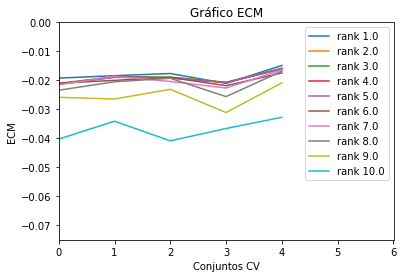
\includegraphics[scale=0.558]{erroresECM}
\centering
\end{figure}

Podemos ver como todos los modelos representados tienen un error por debajo del 4$\%$ de error. Y el modelo elegido es el que en media obtiene el menor error, mostrado en azul oscuro.\\

Podemos decir que este modelo consigue generalizar bien ya que al predecir el conjunto de test que en ningún momento a sido tratado en el entrenamiento conseguimos un error del 1.7108687215650589 $\%$. Mayor que en el conjunto de entrenamiento, pero prácticamente inapreciable.

\subsection{Justificación}

El modelo que he elegido parece representar de forma fidedigna la realidad de los datos. Los errores conseguidos son muy buenos, incluso con la parte de la muestra que no se ha introducido en el entrenamiento, esto parece indicar que cuando lo apliquemos a la población funcionará con un error parecido.\\

Aún así el error cuadrático medio utilizado puede entre ver carencias en el modelo debido a su simplicidad, aunque he elegido este error para tratar de que los valores perdidos no aporten en el ajuste. De esta forma consigo que rellenando los valores con la media estos no se consideren. Aun que este no sea el error real en la población, nos encontramos ante una muy buena cota.\\




\end{document}
